En este capítulo se hablará sobre como se ha desarrollado el proyecto. Para ello primero hablaremos
de la metodología utilizada para después pasara a explicar cuál fue el proceso de desarrollo del sistema.

\section{Metodología}

Para poder escoger una buena metodología tenemos que saber de los recursos que disponemos además
de cuales son nuestros objetivos (funciones a desarrollar en que tiempo). Previamente se hablo
de los objetivos pero un resumen de ellos sería desarrollar una aplicación, con la mayor
accesibilidad posible para ayudar al mundo de la esgrima. Para ello se llegó a la conclusión de que
se desarrollaría un sistema de apoyo a la decisión el cuál tendría una interfaz web, de este modo
se podría acceder a ella desde cualquier sitio con internet. Este proyecto ha de desarrollarse
en un periodo de tiempo de unas 300 horas aproximadas por lo que no podremos llegar a
desarrollarlo por completo, de modo que este será un factor importante a la hora de elegir la metodología.
La que escojamos deberá favorecer el trabajo en funcionalidades completas, de modo que cada vez
que se empiece una, se deberá acabar.

Otra cosa a tener en cuenta son los recursos de los que se dispone. En este caso se dispone de
un desarrollador el cual hará a su vez de Ingeniero del Conocimiento. También se dispone de un
experto en la materia, cuyas horas no serán contabilizadas. Además dichas personas no están a tiempo
completo dedicadas al proyecto, solo podrán dedicarle tiempo de forma ocasional. Esto hace que sea
mas complicado el desarrollo del mismo, por lo que no se podrán tener varias funcionalidades abiertas
sin acabar.

Además sabemos cual es nuestro punto de partida, al igual que nuestra meta, pero el camino es
en su mayoría incierto. Esto hará que sea realmente difícil definir una serie de tareas, con
pasos a seguir, las cuales tengan una duración estimada fiable.

Por todo lo mencionado anteriormente deberemos escoger una metodología de desarrollo ágil, la cual
nos permita adaptarnos a los posibles cambios e inconvenientes que vayan surgiendo en el propio
desarrollo. También deberemos escoger una metodología incremental, la cuál nos permitirá aumentar
los objetivos de la aplicación en cualquier momento del desarrollo.

\section{Extreme Programming}

La metodología utilizada ha sido eXtreme Programming (XP en adelante). Esto es debido a que es una
metodología iterativa-incremental la cual permite el desarrollo de aplicaciones de modo que en cada
iteración aumente la funcionalidad de la misma. Una de las principales ventajas que nos ofrece
es su cercanía a la improvisación. Como se dijo antes necesitaremos una metodología la cual
nos permita improvisar, puesto que desconocemos el camino a seguir. XP también nos facilita
el incremento de funcionalidades con el paso del tiempo, puesto que se centra en sacar versiones
estables del proyecto y no pasar a la siguiente hasta que no este estable. En la figura 4.1 se
puede ver el flujo normal trabajando con extreme programming


\begin{figure}[htb]
  \centering
    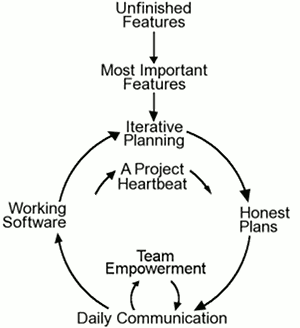
\includegraphics[width=0.4\linewidth]{agileflowchart}
  \caption[Desarrollo SE]{Desarrollo SE}
  \label{fig:Desarrollo Sistema Experto}
\end{figure}



\subsection{Valores}

Los valores que se defienden en esta metodología son los siguientes:

\begin{itemize}
  \item \textbf{Simplicidad:} Esta es la base de XP. Cuanto mas simple sea el diseño, mas sencillo será de programarlo. Es por esto
    por lo que deberemos tener especial atención a las definiciones de los problemas. Para ayudar a un código sencillo se facilitará
    la refactorización de código cuanto sea necesario en cada iteración. De este modo no generaremos un código muy complejo según
    añadamos funcionalidades. La documentación del código no debera ser muy extensa ya que un buen código estará autodocumentado
    y se entenderá por si mismo.
  \item \textbf{Comunicación:} Reforzando el anterior apartado, la comunicación ha de ser sencilla. Evitar los comentarios
    en el código y mejorar este para que se explique automáticamente es algo fundamental. Por otro lado el desarrollo
    de test unitarios facilita la comunicación, puesto que estos explicarán de una manera muy clara los casos de uso.
  \item \textbf{Retroalimentación:} En esta metodología el cliente está muy implicado. Los tiempos en los que se hacen
    desarrollo y se entrega al cliente son muy cortos, de modo que se pueden comprobar funcionalidades poco después
    de desarrollarlas. De este modo evitaremos en gran medida los desarrollos que después de enseñarselos al cliente se desechan.
  \item \textbf{Valentia:} Para esta metodología tenga éxito hay que ser valiente tomando decisiones para que el diseño no se complique
    demasiado, puesto que esto conllevaría mayor tiempo de desarrollo, lo cual haría verse comprometida la faceta de entregas
    en poco tiempo.
  \item \textbf{Respeto:} Todos los miembros del equipo han de ser respetados. Todos los miembros del equipo aportan
    algo a él y no funcionaría sin ellos. Desde la dirección se respetará a dar responsabilidades a cada uno de los miembros.
\end{itemize}

\subsection{Características}

Lo que caracteríza a esta metodología es lo siguiente:

% Cambiar las palabras de esto
\begin{itemize}
  \item \textbf{Desarrollo iterativo e incremental:} pequeñas mejoras, unas tras otras.
  \item \textbf{Pruebas unitarias continuas,} frecuentemente repetidas y automatizadas, incluyendo pruebas de regresión. Se aconseja escribir el código de la prueba antes de la codificación. Véase, por ejemplo, las herramientas de prueba JUnit orientada a Java, DUnit orientada a Delphi, NUnit para la plataforma.NET o PHPUnit para PHP. Estas tres últimas inspiradas en JUnit, la cual, a su vez, se insipiró en SUnit, el primer framework orientado a realizar tests, realizado para el lenguaje de programación Smalltalk.equeñas mejoras, unas tras otras.
  \item \textbf{Programación en parejas:} se recomienda que las tareas de desarrollo se lleven a cabo por dos personas en un mismo puesto. La mayor calidad del código escrito de esta manera -el código es revisado y discutido mientras se escribe- es más importante que la posible pérdida de productividad inmediata.
  \item \textbf{Integración del equipo de programación con el cliente o usuario.} Se recomienda que un representante del cliente trabaje junto al equipo de desarrollo.
  \item \textbf{Corrección de todos los errores} antes de añadir nueva funcionalidad. Hacer entregas frecuentes.
  \item \textbf{Refactorización del código} reescribir ciertas partes del código para aumentar su legibilidad y mantenibilidad pero sin modificar su comportamiento. Las pruebas han de garantizar que en la refactorización no se ha introducido ningún fallo.
  \item \textbf{Propiedad del código compartida:} en vez de dividir la responsabilidad en el desarrollo de cada módulo en grupos de trabajo distintos, este método promueve el que todo el personal pueda corregir y extender cualquier parte del proyecto. Las frecuentes pruebas de regresión garantizan que los posibles errores serán detectados.
  \item \textbf{Simplicidad en el código: } es la mejor manera de que las cosas funcionen. Cuando todo funcione se podrá añadir funcionalidad si es necesario. La programación extrema apuesta que es más sencillo hacer algo simple y tener un poco de trabajo extra para cambiarlo si se requiere, que realizar algo complicado y quizás nunca utilizarlo.
\end{itemize}

Antes del inicio del desarrollo será necesario ponerse de acuerdo con todos los miembros involucrados en el proyecto.
Para ello se utilizará \textit{Agile Inception Deck} el cual estará formado de un conjunto de dinámicas las cuales permitirán
ayudar a llevar al proyecto a la dirección deseada. La parte de \textit{Inception} estará formada por diez preguntas, las
cuales se detallan a continuación:

\begin{enumerate}
  \item \textbf{¿Por qué estamos aquí?}

    Esta cuestión nos permitirá contextualizar el proyecto, respondiendo el motivo del mismo.
  \item \textbf{El \textit{Elevator pitch}}

    Literalmente sería el discurso del ascensor. Este apartado intentará dar respuesta a las preguntas qué, por qué y para qué.
    Para ello se utilizará el símil del tiempo que dura un viaje en el ascensor.
  \item \textbf{Diseñar una caja para el producto}

    Se dará una visión del producto desde la persectiva del cliente.
  \item \textbf{Lista de los no}

    Aquí detallaremos que no es el producto y que no está dentro de él.
  \item \textbf{Conoce a tus vecinos}

    Daremos a conocer a las personas que están involucradas en el proyecto.
  \item \textbf{Muestra la solución}

    Se mostrará la metodología y arquitectura que se utilizará en el desarrollo del proyecto.
  \item \textbf{¿Qué nos quita el sueño por las noches?}

    En este apartado se intentarán predecir los posibles imprevistos surgidos durante
    el desarrollo del proyecto.
  \item \textbf{Tamaño del proyecto}

    Planificación a alto nivel de la duración del proyecto.
  \item \textbf{Muestra con claridad lo que se va a dar}

    Identificar los temas más importantes en el desarrollo del proyecto
  \item \textbf{Muestra lo que va a conllevar}

    Análisis de costes del proyecto.
\end{enumerate}
